\section{RQ2: What Goes Wrong?}
\label{sec:rq2}

\begin{figure}[t]
  \centering
  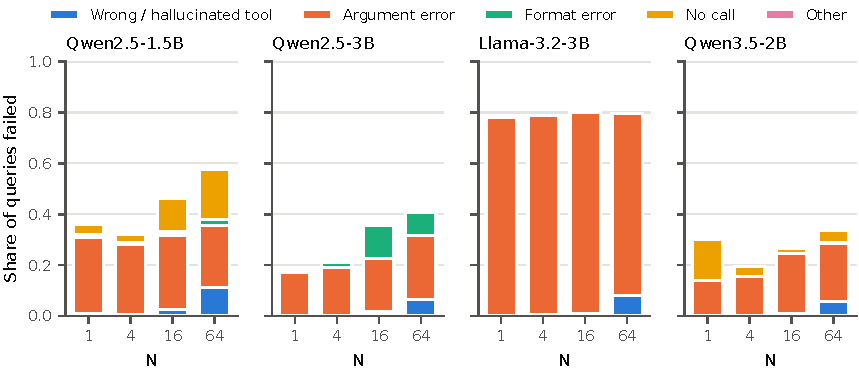
\includegraphics[width=\linewidth]{figures/fig_failures.pdf}
  \caption{Share of queries that fail, by failure group and catalog size (100 queries $\times$ two seeds). \emph{Format error} covers calls with invalid JSON and calls written as prose instead of as a tool call. The full breakdown into categories is in \cref{tab:failures}.}
  \label{fig:failures}
\end{figure}

\begin{table}[t]
  \centering
  \caption{Failure categories (\% of queries) at $N{=}1$ and $N{=}64$. Categories are assigned deterministically from the raw generated tokens (\cref{app:taxonomy}).}
  \label{tab:failures}
  \small
  \begin{tabular}{lrrrrrrrr}
\toprule
Category & \rotatebox{70}{Qwen2.5-1.5B, $N{=}1$} & \rotatebox{70}{Qwen2.5-1.5B, $N{=}64$} & \rotatebox{70}{Qwen2.5-3B, $N{=}1$} & \rotatebox{70}{Qwen2.5-3B, $N{=}64$} & \rotatebox{70}{Llama-3.2-3B, $N{=}1$} & \rotatebox{70}{Llama-3.2-3B, $N{=}64$} & \rotatebox{70}{Qwen3.5-2B, $N{=}1$} & \rotatebox{70}{Qwen3.5-2B, $N{=}64$} \\
\midrule
correct & 64.0 & 42.5 & 83.0 & 58.0 & 22.0 & 20.5 & 70.0 & 66.5 \\
wrong tool & 0.0 & 10.0 & 0.0 & 6.5 & 0.0 & 7.5 & 0.0 & 5.0 \\
hallucinated tool & 1.0 & 1.0 & 0.0 & 0.0 & 0.0 & 0.5 & 0.0 & 0.5 \\
wrong value & 15.0 & 13.0 & 9.0 & 9.5 & 4.0 & 7.0 & 12.0 & 19.5 \\
wrong type & 3.0 & 2.0 & 2.0 & 2.5 & 74.0 & 63.0 & 1.0 & 2.0 \\
missing arg & 6.0 & 5.0 & 1.0 & 5.5 & 0.0 & 1.0 & 0.0 & 1.0 \\
extra arg & 0.0 & 0.5 & 0.0 & 0.0 & 0.0 & 0.0 & 0.0 & 0.0 \\
missing optional & 6.0 & 4.0 & 5.0 & 7.5 & 0.0 & 0.5 & 1.0 & 0.5 \\
malformed call & 0.0 & 1.0 & 0.0 & 9.0 & 0.0 & 0.0 & 0.0 & 0.5 \\
text call & 1.0 & 1.5 & 0.0 & 0.0 & 0.0 & 0.0 & 0.0 & 0.0 \\
no call & 4.0 & 19.5 & 0.0 & 1.5 & 0.0 & 0.0 & 16.0 & 4.5 \\
multi call & 0.0 & 0.0 & 0.0 & 0.0 & 0.0 & 0.0 & 0.0 & 0.0 \\
timeout & 0.0 & 0.0 & 0.0 & 0.0 & 0.0 & 0.0 & 0.0 & 0.0 \\
error & 0.0 & 0.0 & 0.0 & 0.0 & 0.0 & 0.0 & 0.0 & 0.0 \\
\bottomrule
\end{tabular}
\end{table}

It is natural to expect that a larger catalog mainly makes models \emph{pick the wrong tool}. Our taxonomy shows that this is only part of the story (\cref{fig:failures}, \cref{tab:failures}).

\paragraph{Picking the wrong tool grows, but stays small.}
Selection errors (wrong or hallucinated tool) are almost absent up to 16 tools. At $N{=}64$ they reach \FailToolQwenOneFiveNSixtyFour\% (Qwen2.5-1.5B), \FailToolQwenThreeNSixtyFour\% (Qwen2.5-3B), \FailToolLlamaNSixtyFour\% (Llama-3.2-3B) and \FailToolQwenThreeFiveNSixtyFour\% (Qwen3.5-2B).
Most of them pick a \emph{plausible near-duplicate}, because BFCL contains overlapping tools. In a random sample of 14 wrong-tool errors that we inspected by hand, 13 were of this kind (\texttt{solve\_quadratic\_equation} $\to$ \texttt{solve\_quadratic}, \texttt{get\_prime\_factors} $\to$ \texttt{number\_analysis\_prime\_factors}). Only one was unrelated (\texttt{game\_valuation} $\to$ \texttt{book\_hotel}). Some ``errors'' at large $N$ are therefore ambiguity in the benchmark rather than model confusion.

\paragraph{The model stops calling, or breaks the format.}
For Qwen2.5-1.5B, the largest growing category is \emph{no call}: \FailNoCallQwenOneFiveNOne\% at $N{=}1$, \FailNoCallQwenOneFiveNSixtyFour\% at $N{=}64$. Faced with many tools, the model more often answers in text, asks for clarification, or refuses.
For Qwen2.5-3B, the growing category is \emph{format errors}: \FailFormatQwenThreeNOne\% at $N{=}1$, \FailFormatQwenThreeNSixteen\% at $N{=}16$, \FailFormatQwenThreeNSixtyFour\% at $N{=}64$. In \MalformedUnquotedQwenThree{} of its \MalformedNQwenThree{} malformed calls, the function name is written without quotes (\texttt{\{"name": air\_quality, ...\}}). The rest of the call is often correct, but the invalid JSON is \emph{silently discarded} by the serving stack (\cref{sec:discussion}).
Argument errors (wrong values, missing arguments) stay roughly constant with $N$ for the Qwen models. They reflect how hard a query's arguments are to extract, which does not depend on the number of tools.

\paragraph{Too few tools can also hurt.}
Qwen3.5-2B fails \FailNoCallQwenThreeFiveNOne\% of $N{=}1$ queries by answering directly instead of calling the single tool it was given. It works out arithmetic step by step (``the area is 25''), or answers factual questions from memory (``Radium was discovered by Marie Curie''). This drops to \FailNoCallQwenThreeFiveNFour\% at $N{=}4$. A catalog of several tools seems to signal that tool use is expected.

\paragraph{Serialisation dominates Llama-3.2-3B.}
\FailArgLlamaNOne\% of Llama's $N{=}1$ queries fail with argument errors, almost all wrong \emph{types} caused by string-encoded numbers. This is a property of the model plus its chat template, not of tool selection. Whether a deployment notices it depends entirely on whether the tool executor coerces types.
